% HIV contrast --- plan \S4.14 (Phase 4, FULL DETAIL by decision).
% Sources: new_notes2 \S11 (Hataye findings, stage equations, what to
% keep/not claim) and \S13 (linear vs exponential intracellular growth);
% new_notes3 Part G \S30--\S32; paper.pdf = Hataye et al. 2019.
% Notation: latent class L_0 (not L, the flooding parameter); pathway
% conversion \alpha_A, \alpha_B; Erlang per-step rate \alpha; eclipse
% division/death \rho_{\rm div}, \mu_E.

\section{Contrast with HIV: what not to claim}
\label{sec:hiv}

The core results of this chapter are written for pathogens whose
intracellular life ends in load-proportional catastrophe --- lyse and dump.
The motivating applications (\yp{}, \ft{}, lytic phage) are of that kind.
HIV is not: it buds from the plasma membrane, and an infected cell need not
rupture and empty itself in one event. Yet single-cell and
limiting-dilution data show something that looks surge-like --- long quiet
periods, then a concentrated bout of release --- which is exactly the
phenomenon the BDC explains. The honest position is neither to force HIV
into the pure BDC nor to retreat to constant-$p$ BMVR, but to build an
eclipse-structured, short-productive-pulse model on the same renewal
skeleton. This section records what the best data support, gives candidate
equations, and draws the boundary of the chapter's claims.

\subsection{What Hataye et al.\ (2019) show}

Hataye and co-authors \cite{hataye2019principles} coupled
limiting-dilution latency-reactivation cultures to stochastic models, and
their findings --- summarised here at the level that bears on equation
choice --- fall in two groups.

\paragraph{On initial release (viral inhibition cultures; no de novo
infection).}
\begin{enumerate}
\item The timing and magnitude of first HIV RNA release from reactivated
latently infected CD4 T cells are highly variable: total yield, delay to
first detection, and detection duration all fluctuate.
\item Mean release is delayed: first detection most often around day~3,
with a sudden bulk of production around days 3--5 --- not a flat continuous
drip from day~0.
\item A simple productive-cell model (release at constant rate $p$, death
at rate $\delta_{I}$, total yield geometric with mean $p/\delta_{I}$) is
under-dispersed relative to the data: the Fano factor is too small.
\item A single exponential eclipse $E\to I$ fits the delay poorly (its mode
sits at day~1). A multi-stage eclipse --- an Erlang-like chain of $n$
compartments, with $n\approx5$ favoured --- fixes the mean timing.
\item Multi-stage eclipse alone still under-disperses, and transcriptional
ON/OFF toggling does not fix the dispersion under realistic CD4
division/death rates ($\rho_{\rm div}\approx\mu_E\approx0.5/$day from CFSE
and population stability data).
\item Their best structure (``Model~3'') uses two distinct eclipse paths
(high- and low-release potential), multi-stage delay, and division/death in
eclipse. Then: many stimulated lineages release nothing detectable
($f_{\rm HIV}\approx0.41$ of single latently infected cells give detectable
virus in their fit); most productive sojourns last on the order of a day;
and multi-day ``sustained'' detection is largely proliferation in eclipse
followed by staggered short $E\to I$ transitions of descendants --- not one
cell budding steadily for a week.
\end{enumerate}

\paragraph{On establishment (outgrowth cultures; de novo infection
allowed).}
\begin{enumerate}
\item Release of replication-competent virus often fails to establish
exponential spread.
\item Establishment probability as a function of the expected number of
virus-releasing cells per well is sigmoid, not the concave curve of
independent per-cell success --- interpreted as an Allee effect, synergy at
low census.
\item A critical threshold sits near $\Lambda\approx2.3$ latently infected
cells, corresponding on average to roughly $5100$ detected HIV RNA copies
of initial release (under their establishment definition of
$\ge2\times10^5$ copies).
\item For exactly one stimulated latently infected cell, their fitted
dynamics predict establishment only on the order of $2\%$ of the time ---
consistent with the known gap between intact provirus counts and
quantitative viral outgrowth.
\end{enumerate}

\begin{center}
\renewcommand{\arraystretch}{1.25}
\small
\begin{tabular}{@{}p{0.46\textwidth}p{0.46\textwidth}@{}}
\toprule
Supported for HIV & Not supported as literal HIV \\
\midrule
Multi-stage eclipse (delay) & Pure one-type BDC terminal catastrophe \\
Short productive pulse then cell death & Memoryless constant-$p$ BMVR from $t=0$ \\
High stochasticity; many silent lineages & Independent branching alone near threshold \\
Renewal / stage structure for free virus & QSD $=$ geometric burst size as an HIV law \\
Allee / synergistic establishment & \\
\bottomrule
\end{tabular}
\end{center}
The visual ``surge'' is real, but in their best model it is delay plus
brief constant-rate production plus latent lineage dynamics --- not a
single lytic dump of intracellular load.

\begin{center}
\renewcommand{\arraystretch}{1.2}
\small
\begin{tabular}{@{}lll@{}}
\toprule
 & Lytic BDC (this chapter) & HIV (Hataye-guided) \\
\midrule
Release mechanism & catastrophe at rate $\delta X$ & budding while productive \\
End of production & terminal; process absorbed & short productive life; cell dies \\
Intracellular load $X$ & explicit birth--death state & not required as primary state \\
Quiet period & until first catastrophe & multi-stage eclipse ($+$ latency) \\
Sustained multi-day release & one large dump (or nothing) & often staggered short pulses \\
Establishment theory & independent offspring as baseline & Allee synergy near threshold \\
Natural hosts & \yp{}, \ft{}, phage & CD4 T-cell latency / rebound \\
\bottomrule
\end{tabular}
\end{center}

\subsection{Candidate HIV stage equations}
\label{sec:hiv-eqns}

A compact Hataye-aligned system, suitable for coupling to the renewal
free-virus layer of Result~\ref{res:new-vde} (Figure~\ref{fig:hiv-stages}).
Let $L_0$ be a stimulated
latently infected cell (or the start of reactivation). Two eclipse pathways
run in parallel: $A$, of high release potential and multi-stage, and $B$,
low and brief:
\begin{equation}
L_0\xrightarrow{\alpha_A}E_1^{(A)},
\qquad
L_0\xrightarrow{\alpha_B}E^{(B)},
\end{equation}
\begin{equation}
E_j^{(A)}\xrightarrow{\alpha}E_{j+1}^{(A)}\ (j=1,\dots,n-1),
\qquad
E_n^{(A)}\xrightarrow{\alpha}I^{(A)},
\qquad
E^{(B)}\xrightarrow{\alpha_B}I^{(B)}.
\end{equation}

\begin{figure}[H]
\centering
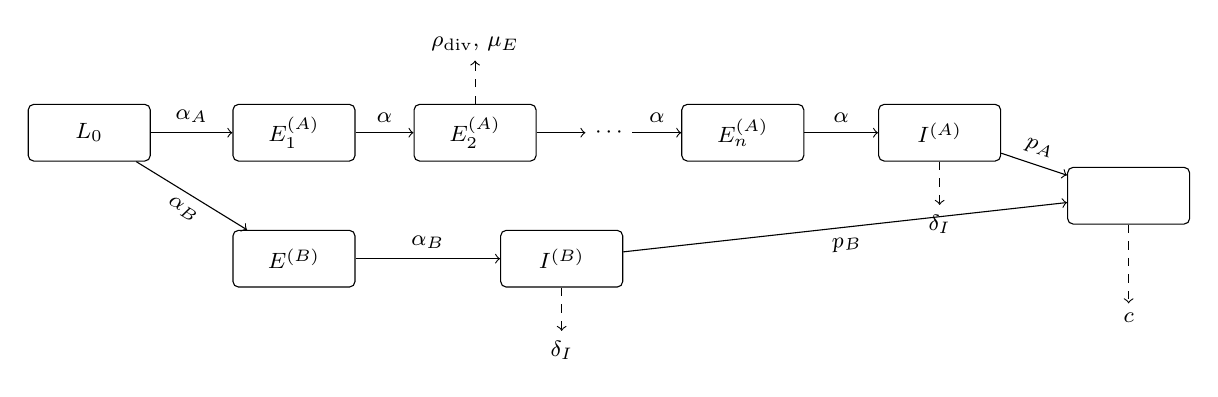
\begin{tikzpicture}[font=\footnotesize,
  box/.style={draw,rounded corners=2pt,minimum height=0.72cm,
              minimum width=1.55cm,align=center}]
% pathway A (upper)
\node[box] (L0)  at (0,1.6) {$L_0$};
\node[box] (E1)  at (2.6,1.6) {$E_1^{(A)}$};
\node[box] (E2)  at (4.9,1.6) {$E_2^{(A)}$};
\node      (Ed)  at (6.6,1.6) {$\cdots$};
\node[box] (En)  at (8.3,1.6) {$E_n^{(A)}$};
\node[box] (IA)  at (10.8,1.6) {$I^{(A)}$};
% pathway B (lower)
\node[box] (EB)  at (2.6,0) {$E^{(B)}$};
\node[box] (IB)  at (6.0,0) {$I^{(B)}$};
% free virus
\node[box] (V)   at (13.2,0.8) {$\Vfree$};
% arrows
\draw[->] (L0) -- node[above,sloped] {$\alpha_A$} (E1);
\draw[->] (E1) -- node[above] {$\alpha$} (E2);
\draw[->] (E2) -- (Ed);
\draw[->] (Ed) -- node[above] {$\alpha$} (En);
\draw[->] (En) -- node[above] {$\alpha$} (IA);
\draw[->] (L0) -- node[below,sloped] {$\alpha_B$} (EB);
\draw[->] (EB) -- node[above] {$\alpha_B$} (IB);
\draw[->] (IA) -- node[above,sloped] {$p_A$} (V);
\draw[->] (IB) -- node[below,sloped] {$p_B$} (V);
% losses
\draw[->,dashed] (IA.south) -- ++(0,-0.55) node[below] {$\delta_I$};
\draw[->,dashed] (IB.south) -- ++(0,-0.55) node[below] {$\delta_I$};
\draw[->,dashed] (E2.north) -- ++(0,0.55)
  node[above] {$\rho_{\rm div},\,\mu_E$};
\draw[->,dashed] (V.south) -- ++(0,-1.0) node[below] {$c$};
\end{tikzpicture}
\caption{The Hataye-aligned stage structure of \S\ref{sec:hiv-eqns}: two
eclipse pathways from the stimulated latent class $L_0$ --- a multi-stage
path $A$ of high release potential and a brief path $B$ --- each feeding a
short productive class that releases at constant rate; division and death
(dashed) act in eclipse, death $\delta_I$ in the productive classes, and
clearance $c$ on free virus.}
\label{fig:hiv-stages}
\end{figure}

In each eclipse compartment, cells may divide or die without releasing
virus,
\begin{equation}
E\xrightarrow{\rho_{\rm div}}E+E,
\qquad
E\xrightarrow{\mu_E}\varnothing,
\end{equation}
with $\rho_{\rm div}\approx\mu_E\approx0.5/$day in the Hataye fits.
Productive cells release at constant rate and die,
\begin{equation}
I^{(A)}\xrightarrow{p_A}I^{(A)}+\Vfree,
\qquad
I^{(A)}\xrightarrow{\delta_I}\varnothing,
\qquad
I^{(B)}\xrightarrow{p_B}I^{(B)}+\Vfree,
\qquad
I^{(B)}\xrightarrow{\delta_I}\varnothing,
\end{equation}
with $p_A\gg p_B$ (or $p_B$ small and $I^{(B)}$ short-lived) to match the
bimodal release distribution; free virus clears at rate $c$. The
mean-field stage ODEs (large inoculum $\Lambda$, suppressing the dual path
for display) are
\begin{equation}
\ddt{E_1}=\alpha_A L_0\,\delta_0(t)+\rho_{\rm div}E_1
-(\mu_E+\rho_{\rm div}+\alpha)E_1,
\end{equation}
\begin{equation}
\ddt{E_j}=\alpha E_{j-1}+\rho_{\rm div}E_j
-(\mu_E+\rho_{\rm div}+\alpha)E_j,\quad j=2,\dots,n,
\end{equation}
\begin{equation}
\ddt{I^{(A)}}=\alpha E_n-\delta_I I^{(A)},
\qquad
\ddt{\Vfree}=p_A I^{(A)}-c\,\Vfree
\quad(+\,p_B I^{(B)}),
\end{equation}
where the Dirac source stands for an initial cohort; for ongoing infection
it is replaced by incidence, split between pathways with
$\pi_A+\pi_B=1$:
\begin{equation}
i(t)=f\bigl(\Vfree(t),T\bigr),
\qquad
\text{source into }E_1^{(A)}=\pi_A i(t),
\qquad
\text{source into }E^{(B)}=\pi_B i(t).
\end{equation}
Linear infection (the classical, large-population limit) takes
$f(\Vfree,T)=\gamma T\,\Vfree$ and recovers a stage-structured BMVR. Near
the establishment threshold, however, the Hataye data favour a sigmoid law
over independent per-virion success; a minimal phenomenological upgrade is
the Allee incidence
\begin{equation}
f(\Vfree,T)=\gamma T\,\Vfree\cdot\frac{\Vfree}{K_A+\Vfree},
\end{equation}
inefficient at very low $\Vfree$ and saturating to mass action for
$\Vfree\gg K_A$, with $K_A$ chosen so that cumulative initial release near
$\sim5\times10^3$ RNA copies sits at the inflection of establishment
probability --- the empirical threshold above. More mechanistic forms
(cooperative entry, restriction-factor saturation, local multiplicity) can
replace it; the point is that linearity in $\Vfree$ alone is not faithful
near establishment.

Coupled to free virus, the stage model induces renewal kernels of the usual
kind. Let $g_{\rm HIV}(a)$ be the expected release rate at age $a$ after a
single infection or reactivation, and $S_{\rm HIV}(a)$ the probability of
still being in a productive (or not-yet-cleared) lineage. Then exactly the
skeleton \eqref{eq:skeleton} holds:
\begin{equation}
\Icell(t)=\Icell_0S_{\rm HIV}(t)+(i*S_{\rm HIV})(t),
\qquad
\ddt{\Vfree}=\Icell_0g_{\rm HIV}(t)+(i*g_{\rm HIV})(t)-c\,\Vfree(t).
\end{equation}
For the stage model, $g_{\rm HIV}$ is \emph{not} $\delta K$: it is the
density of productive sojourn times times $p_A$ (and $p_B$), with the
Erlang eclipse supplying the delay --- $g_{\rm HIV}(a)\approx0$ for small
$a$, then rising and falling: the mathematical expression of ``nothing for
a long time, then a lot''. The effective parameters of
\S\ref{sec:peff-section} carry over by the substitution
$(\Ihat,g)\mapsto(S_{\rm HIV},g_{\rm HIV})$:
\begin{equation}
p_{\rm eff}(r)=\frac{\Lap{g}_{\rm HIV}(r)}{\Lap{S}_{\rm HIV}(r)},
\qquad
R_0=\frac{\gamma T}{c}\int_0^\infty g_{\rm HIV}(a)\,\dd a
\quad\text{(linear incidence)},
\end{equation}
while under the Allee form $R_0$ remains the large-population threshold and
early establishment is governed in addition by the scale $K_A$.

\subsection{What to keep, what not to claim}

\begin{itemize}
\item \textbf{Keep} for HIV: the renewal free-virus coupling; age/stage
kernels; the lesson that constant $p$ is only an exponential-phase
projection; stochastic early failure; eclipse as a real dynamical object
(the GATE mechanism of Chapter~5, multi-stage here).
\item \textbf{Do not claim} for HIV: terminal catastrophe at rate
$\delta X$; QSD $=$ geometric burst size as an HIV law; one-shot
cumulative release as the only single-cell trajectory; independent
branching as the full establishment story near the Hataye threshold.
\item \textbf{Flooding comparison:} still meaningful as a \emph{linear}
baseline --- matched mean yield, compare offspring variance --- but near
$\sim5\times10^3$ RNA copies synergy can dominate variance effects, and any
HIV write-up should separate the two mechanisms.
\end{itemize}

\subsection{HIV intracellular mean growth: linear vs exponential}
\label{sec:hiv-growth}

One modelling decision underlies the stock-and-export cases of
\S\ref{sec:five-cases} and deserves its own statement: does the mean
intracellular load grow exponentially (birth--death) or linearly
(template-limited production)?

\begin{center}
\renewcommand{\arraystretch}{1.2}
\small
\begin{tabular}{@{}lll@{}}
\toprule
Regime & Mean law & Mechanism \\
\midrule
Mean-exponential & $m'=r\,m$ & each unit generates more units (branching / BDC) \\
Mean-linear & $m'\approx\nu-\mu m$ & production set by fixed templates / machinery \\
\bottomrule
\end{tabular}
\end{center}
Absorbing BDC and pure birth--death are exponential-mean; immigration and
constant production are linear-mean. HIV does \emph{not} amplify infectious
units inside the cell by branching: after integration the DNA template
count is typically one or a few proviruses, not an exponentially growing
genome pool; late genomic RNA is made by host Pol~II from that fixed
template, not by cytoplasmic genome cascading; and Gag and the other
structural products are translated from mRNA and do not self-replicate.
Production is immigration-like: rate set by mRNA and ribosomes, minus
degradation, packaging and export. Pure $m'=rm$ is a poor literal
description of HIV intracellular load; it fits phage genome races,
intracellular bacterial division, and some cytoplasmic RNA viruses far
better. The main nonlinearity is Tat positive feedback: transcription rises
from a low basal level towards a saturated high state. During the switch,
product counts can rise faster than a pure linear ramp, because the
\emph{production rate} is increasing --- not because each unit is a
branching particle; and once fully ON, production is roughly constant about
a high mean, so mean accumulation is linear or saturating. The late
fully-ON rate is the ceiling, and the intermediate phase climbs towards it;
in the mean it does not systematically exceed it (stochastic
transcriptional bursts can spike above the late \emph{mean} rate, but that
is noise, not a hotter phase; and net accumulation can peak mid-course if
export turns on late, but that is export balance, not Tat overshoot).
Confidence: high that HIV is not pure exponential-mean birth--death of
virion-like units; medium--high that the main productive window is closer
to mean-linear than exponential; medium on the exact shape of $m(a)$, which
depends on the molecular species counted and on the Tat phase. The
recommended coarse regime is therefore
\begin{equation}
\textbf{eclipse}\ \longrightarrow\
\textbf{mean-linear (immigration-type) accumulation of }X,
\end{equation}
with a fixed or multi-step delay so first activity is not peaked at
$t=0^+$, production $m'\approx\nu-\mu m$ (or $m'\approx\nu$ while
accumulating) at the late fully-ON rate $\nu$, Tat switch-on folded into a
slightly longer eclipse plus an abrupt start of $\nu$, and the export law
left open --- the linear-vs-exponential choice for accumulation does not
force it. In ranking: birth--death / absorbing BDC fits poorly as a literal
HIV mechanism; immigration plus export or dump is a much better caricature;
eclipse then constant production rate is the best simple default; Tat ON/OFF
plus immigration the best simple mechanistic default.

\subsection{Suggested role of this material}

The core lytic results stand as the chapter's contribution; this section is
their honest boundary. In a companion paper the natural order is: the BDC
and renewal results at the lytic end of the spectrum; then ``HIV is not
BDC'', with Hataye's Model~3 as the empirical intermediate and the stage
equations above; then numerical extraction of $g_{\rm HIV}(a)$ from the
stage model (or from daily release curves), overlaid against constant-$p$
BMVR exactly as in \S\ref{sec:overlays}; and finally establishment by
independent branching vs the Allee form, with the critical release scale
taken from experiment.
